\section{Rekonstruktion toteutus}
Säteen lävistämien kuva-alueen vokseleiden laskentaan Siddonin algoritmilla tarvitaan kaksi pistettä säteen virittämältä suoralta avaruudessa kuva-alueen parametrien lisäksi\cite{sundermann_fast_1998}. Koska epäideaalin kollimaattorin reikä kerää säteilyä kartion muotoiselta alueelta avaruudessa\cite{cherry_single_2012}, jokaiselle detektorin pikselille asetetaan useampi säde kollimaattorin reikien sisälle. Kunkin säteen lävistämät vokselit ja pituudet niissä määritetään, jonka jälkeen pituudet keskiarvoistetaan vokselikohtaisesti. Projektion lasketaan käytetään näitä keskiarvoja.

\subsection{Kollimaattorin mallinnus}
Työssä toteutettiin kaksi eri mallia kollimaattorille, jonka reiät ovat suoria särmiöitä kuusikulmaisella pohjalla. Toinen malli on kehitetty mahdollisimman todenmukaista rekonstruktiota varten ja toinen laskentatehokkuutta ajatellen.

Kummassakin mallissa kollimaattorin yksittäisen reiän ajatellaan koostuvan sisäkkäisistä kuusikulmaisista suorista särmiöistä. Jokaiselle särmiölle muodostetaan kuusi avaruuslävistäjää, jotka toimivat projektion laskennassa tarvittavina säteinä. Ennen laskentaa kuitenkin tarkistetaan vielä, että säteet osuvat oikeaan pikseliin detektorissa. \hyperref[fig:ray1]{Kuva \ref*{fig:ray1}} havainnollistaa detektoripaneelin tasoa ja kollimaattorin malleja. Tasolle on rajattu detektorin pikselit punaisella viivalla ja säteiden päätepisteet sinisillä pisteillä.

\begin{figure}[t]
    \centering
    \captionsetup{width=.9\textwidth}
    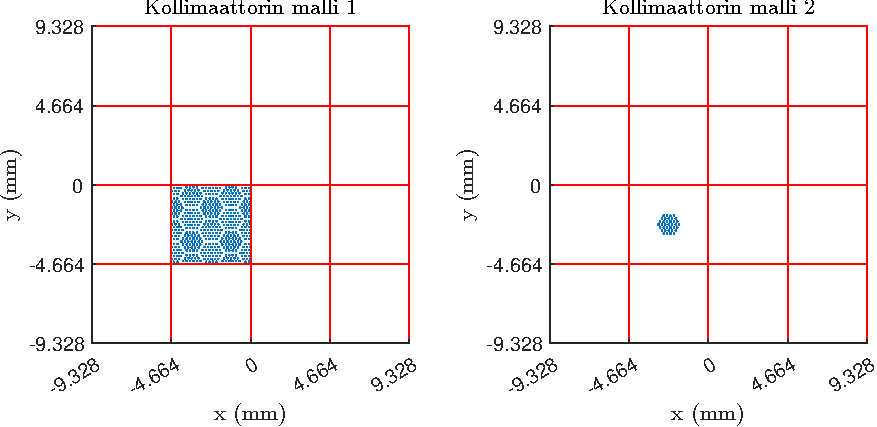
\includegraphics[width=.9\textwidth]{kuvat/2d-kollimaattori.pdf}
    \caption{Detektoripaneelin taso. Detektorin pikselit ovat rajattu punaisilla viivoilla ja kollimaattorin reikien sisälle yhden pikselin alueella on asetettu tasaisesti pisteitä sinisellä värillä. Vasemmalla puolella, mallissa 1, säteitä on 543 ja oikealla puolella, mallissa 2, säteitä on 37. Kollimaattorin reiän halkaisija on \qty{1.4}{\milli\meter} ja reikien väli on \qty{0.12}{\milli\meter}. Detektorin pikselin koko on \qty{4.664}{\milli\meter}.}
    \label{fig:ray1}
\end{figure}

Ensimmäisessä mallissa kollimaattorin reiät ovat todenmukaisissa paikoissaan. \hyperref[fig:ray1]{Kuvan \ref*{fig:ray1}} vasemmassa laidassa esitetty malli sisältää 543 sädettä, kun yhdessä kollimaattorin reiässä on 37 sädettä. \hyperref[fig:ray1]{Kuvan \ref*{fig:ray1}} oikeassa laidassa esitetty toinen malli muodostuu vain yhdestä kollimaattorin reiästä detektorin pikseliä kohti. 

Kuviin \ref{fig:ray2} ja \ref{fig:ray3} on piirretty kuva-alue kolmiulotteisessa avaruudessa mustalla ruudukolla ja detektorin yhdelle pikselille asettuvat säteet sinisillä viivoilla. \hyperref[fig:ray2]{Kuvassa \ref*{fig:ray2}} on käytetty todenmukaisempaa mallia 98 säteellä, jolloin jokaista kollimaattorin reikää kohti jää 7 sädettä. Seitsemän säteen kuvio on selvästi nähtävissä suuremmassakin mittakaavassa.

\begin{figure}[H]
    \centering
    \captionsetup{width=.9\textwidth}
    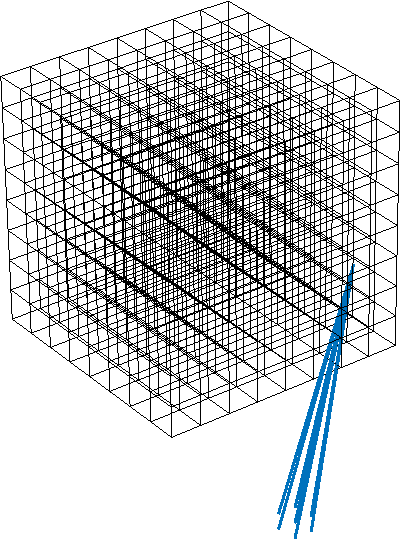
\includegraphics[height=6cm]{kuvat/3d-kollimaattori1.pdf}
    \caption{Kollimaattorin mallin 1 havainnollistus kolmiulotteisessa avaruudessa. Kuva-alue on piirretty mustalla ruudukolla ja detektorin havaitsemat säteet (98 kappaletta) sinisellä värillä. Kollimaattorin reiän pituus on \qty{32.4}{\milli\meter}, reiän halkaisija on \qty{1.4}{\milli\meter} ja reikien välinen etäisyys on \qty{0.12}{\milli\meter}. Detektorin pikselin koko on \qty{4.664}{\milli\meter}. Yksi ruudukon kuutio vastaa $8^3$ vokselia, jossa yksittäisen vokselin koko on $(\qty{4.664}{\milli\meter})^{3}$.}
    \label{fig:ray2}
\end{figure}

\hyperref[fig:ray3]{Kuvassa \ref*{fig:ray3}} on esitetty jälleen kuva-alue mustalla ruudukolla ja detektorin yhdelle pikselille asettuvat säteet sinisillä viivoilla. Kuvaan on piirretty yhteensä 61 sädettä mallilla 2. Kuvista nähdään, kuinka detektorin havaitsema alue avaruudesta täyttyy tasaisemmin yhden reiän mallilla, vaikka säteitä on yli kolmannes vähemmän.

\begin{figure}[H]
    \centering
    \captionsetup{width=.9\textwidth}
    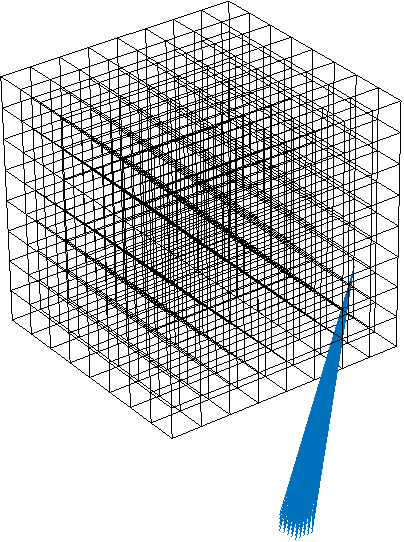
\includegraphics[height=6cm]{kuvat/3d-kollimaattori2.pdf}
    \caption{Kollimaattorin mallin 2 havainnollistus kolmiulotteisessa avaruudessa. Kuva-alue on piirretty mustalla ruudukolla ja detektorin havaitsemat säteet (61 kappaletta) sinisellä värillä. Kollimaattorin reiän pituus on \qty{32.4}{\milli\meter}, reiän halkaisija on \qty{1.4}{\milli\meter} ja reikien välinen etäisyys on \qty{0.12}{\milli\meter}. Detektorin pikselin koko on \qty{4.664}{\milli\meter}. Yksi ruudukon kuutio vastaa $8^3$ vokselia, jossa yksittäisen vokselin koko on $(\qty{4.664}{\milli\meter})^{3}$.}
    \label{fig:ray3}
\end{figure}

\subsection{Koodin toiminta}
Kollimaattorin mallintava koodi kehitettiin MATLAB-ympäristössä (R2023b, Mathworks Inc.) testauksen nopeuden ja helppouden vuoksi. Toimivassa versiossa hyödynnettiin eräitä MATLABin funktioita, joita ei ole C++:n vakiokirjastossa. Näitä ovat muun muuassa trigonometriset funktiot, joiden argumenttina on kulma asteina sekä funktio \texttt{floorDiv}, joka laskee ensin kahden luvun osamäärän ja pyöristää sen alaspäin lähimpään kokonaislukuun. Koodin luettavuuden kannalta on helpompaa toteuttaa nämä erillisinä apufunktioina C++:ssa. Apufunktiot kokonaisuudessaan ovat esitetty \hyperref[appendix:apufunktiot]{liitteessä \ref*{appendix:apufunktiot}}.

Koska kummallekin mallille on yhteistä se, kuinka säteet asettuvat kollimaattorin yksittäiseen reikään, oli luontevaa eriyttää säteiden päätepisteiden asettava funktio omakseen. \hyperref[appendix:2Dsiirto]{Liitteen \ref*{appendix:2Dsiirto}} funktio \texttt{computeHexShifts2D} asettaa säännöllisen kuusikulmion sisälle $n\in\NN$ pistettä.

Funktiolle \texttt{computeHexShifts2D} annetaan parametreinä pisteiden lukumäärä \texttt{nPoints}, kuusikulmion kärjen ja $x$-akselin välinen kulma \texttt{startAngle} ja kuusikulmion halkaisija \texttt{diameter}. Funktio palauttaa listan pisteistä $(x, y)\in\RR^2$, jotka vastaavat kuusikulmioon sijoittuvien pisteiden koordinaatteja. Tämä lista, C++:n vakiokirjaston vektori \texttt{hexShifts}, alustetaan rivillä 3. Riveillä 4-6 tarkistetaan, onko kuusikulmioon asetettavien pisteiden lukumäärä 1. Jos näin on, niin ainut palautettava piste on kuusikulmion keskipiste $(0, 0)$. Rivillä 8 asetettu muuttuja \texttt{currentPoint} pitää kirjaa siitä, kuinka monta pistettä vektoriin \texttt{hexShifts} on jo lisätty. Seuraavalla rivillä asetetaan kuusikulmion säteelle apumuuttuja \texttt{radius}, jotta sädettä ei tarvitse laskea kuin kerran.

Kun kuusikulmio jaetaan tasasivuisiin kolmioihin, kolmioiden kärkipisteistä saadaan tasaisesti jakautuneita pisteitä kuusikulmion sisällä. Kolmioiden määrityksessä kuusikulmio on jaettu useampaan kerrokseen, joista jokaista rajaa kaksi sisäkkäistä kuusikulmiota. Periaate on esitetty \hyperref[fig:6kulmio]{Kuvassa \ref*{fig:6kulmio}} eri kerrosten lukumäärällä. Kuvan vasemmassa laidassa kerroksia on nolla, eli ainoa piste on kuusikulmion keskipiste. Oikealle päin seuraavassa kuvassa kerroksia on yksi eli pisteet ovat kuusikulmion keskipiste ja kaikki kulmat. Seuraavassa kuvassa kerroksia on kaksi, josta nähdään, kuinka voidaan muodostaa 24 tasasivuista kolmiota. Kärkipisteitä näillä kolmioilla on yhteensä 19. Oikeanpuolimmaisessa kuvassa kerroksia on kolme, jolloin kuusikulmio jakautuu 54 tasasivuiseen kolmioon ja 37 kärkipisteeseen.
\begin{figure}[H]
    \centering
    \captionsetup{width=.9\textwidth}
    \begin{subfigure}[t]{.225\textwidth}
        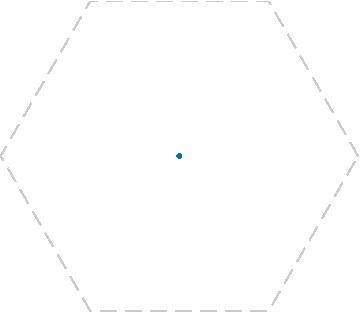
\includegraphics[width=.9\linewidth]{kuvat/6kulmio0.pdf}
        \caption{}
    \end{subfigure}%
    \begin{subfigure}[t]{.225\textwidth}
        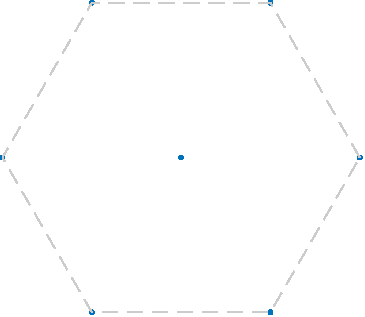
\includegraphics[width=.9\linewidth]{kuvat/6kulmio1.pdf}
        \caption{}
    \end{subfigure}%
    \begin{subfigure}[t]{.225\textwidth}
        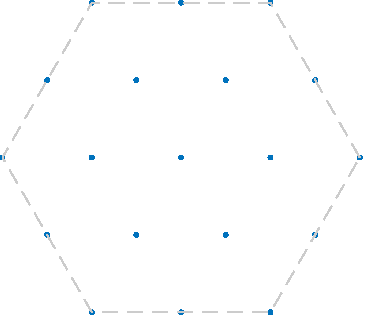
\includegraphics[width=.9\linewidth]{kuvat/6kulmio2.pdf}
        \caption{}
    \end{subfigure}%
    \begin{subfigure}[t]{.225\textwidth}
        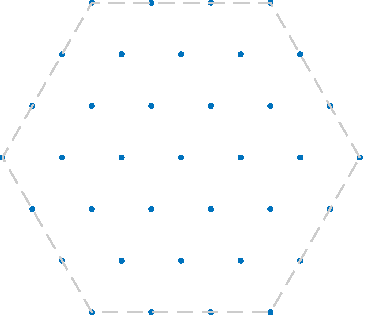
\includegraphics[width=.9\linewidth]{kuvat/6kulmio3.pdf}
        \caption{}
    \end{subfigure}%
    \caption{Kuusikulmion jakaminen kerroksiin. Harmaa katkoviiva kuvaa kuusikulmion kehää. Siniset pisteet ovat kuusikulmion jakavien tasasivuisten kolmioiden kärkipisteitä.}
    \label{fig:6kulmio}
\end{figure}

Havaitaan, että kerrosten lukumäärän $k$ lisääntyessä yhdellä, olettaen $k>0$, pisteiden lukumäärä lisääntyy $6k$:lla. Siis, jos kerroksia on $k$ kappaletta, niin pisteitä on
\begin{equation}\label{eqn:pisteidenlkm}
    n=1+\sum\limits_{i=0}^{k}6i
\end{equation}
kappaletta. Koska funktiolle \texttt{computeHexShifts2D} syötetään pisteiden lukumäärä, tasaista asettelua varten täytyy määrittää pienin kerrosten lukumäärä $k$, jolle kaikki pisteet mahtuvat. Käytännössä yhtälöstä (\ref{eqn:pisteidenlkm}) täytyy ratkaista muuttuja $k$, joka tapahtuu aritmeettisen summan osasumman\cite{harjulehto_analyysia_2022} avulla. Osasummasta saadaan
\begin{equation*}
    n-1=6\frac{k(k+1)}{2},
\end{equation*}
joka on muuttujan $k$ toisen asteen yhtälö. Yhtälön juuret ovat
\begin{equation*}
    k=\frac{1}{2}\left( \pm\sqrt{4\cdot\frac{n - 1}{3} + 1} - 1 \right)
\end{equation*}
ja koska kerrosten lukumäärän täytyy olla epänegatiivinen, saadaan
\begin{equation*}
    k=\frac{1}{2}\left( \sqrt{4\cdot\frac{n - 1}{3} + 1} - 1 \right).
\end{equation*}
Kerrosten lukumäärän täytyy olla myös kokonaisluku, joten pyöristetään kerrosten lukumäärä ylöspäin lähimpään kokonaislukuun. Siten
\begin{equation}\label{eqn:kerrostenlkm}
    k=\left\lceil\frac{1}{2}\left( \sqrt{4\cdot\frac{n - 1}{3} + 1} - 1 \right)\right\rceil.
\end{equation}
Yhtälö (\ref{eqn:kerrostenlkm}) on toteutettu funktion \texttt{computeHexShifts2D} rivillä 10.

Riveillä 12 ja 13 asetetaan tilapäiset muuttujat kuusikulmion pisteen sijainnille. Riviltä 15 eteenpäin käydään läpi jokainen kuusikulmion kerros, jokaisen kerroksen kärki ja asetetaan tilapäisten muuttujien arvoiksi kärjen sijainti. Kerroksella $k$, $k>0$, tilapäistä muuttujaa siirretään $6k$ kertaa tasaisin välein ja pisteet tallennetaan vektoriin \texttt{hexShifts}. Joka lisäyksellä tarkistetaan, onko vektori \texttt{hexShifts} täynnä. Jos on, niin vektori palautetaan.

Parametreinä kummassakin mallissa ovat detektorin pikselin koko, pikselin indeksi detektoripaneelissa, kollimaattorin reiän halkaisija, reiän pituus, reikien välinen etäisyys (\textit{septal width}), kuusikulmaisen reiän suuntaus ja säteiden lukumäärä. Reiän suuntauksessa arvo 1 asettaa kuusikulmion kärjet detektoripaneelin tason $x$-akselin suuntaisesti ja arvo 2 $y$-akselin suuntaisesti.

Pääfunktion \texttt{computeSpectHexShifts} parametrit ovat esitetty myös \hyperref[tbl:parametrit]{Taulukossa \ref*{tbl:parametrit}}.
\begin{table}[H]
    \centering
    \captionsetup{width=.9\textwidth}
    \caption{Funktion \texttt{computeSpectHexShifts} parametrit}
    \resizebox{.9\textwidth}{!}{%
        \begin{tabular}{lcc}
            \toprule
            Parametrin nimi & Arvo & Kuvaus \\
            \midrule
            \texttt{param.coneMethod} & $\left\{ 1, 2 \right\}$ & Mallin valinta \\
            \texttt{param.hexOrientation} & $\left\{ 1, 2 \right\}$ & Kuusikulmion pohjan suuntaus \\
            \texttt{param.nRaySPECT} & $\mathbb{N}$ & Säteiden lukumäärä yhdessä kollimaattorin reiässä \\
            \texttt{param.dPitchXY} & $>0$ & Detektorin pikselin reunan pituus \\
            \texttt{param.colL} & $>0$ & Kollimaattorin reiän pituus \\
            \texttt{param.colD} & $>0$ & Kollimaattorin reiän halkaisija \\
            \texttt{param.dSeptal} & $>0$ & Kollimaattorin reikien välinen etäisyys \\
            \texttt{detectors.xd} & $\mathbb{R}$ & Detektorin pikselin keskipisteen $x$-koordinaatti \\
            \texttt{detectors.yd} & $\mathbb{R}$ & Detektorin pikselin keskipisteen $y$-koordinaatti \\
            \texttt{detectors.zd} & $\mathbb{R}$ & Detektorin pikselin keskipisteen $z$-koordinaatti \\
            \texttt{detectors.xs} & $\mathbb{R}$ & \texttt{detectors.xd} + detektoripaneelin ulkonormaalivektorin $x$-komponentti \\
            \texttt{detectors.ys} & $\mathbb{R}$ & \texttt{detectors.yd} + detektoripaneelin ulkonormaalivektorin $y$-komponentti \\
            \texttt{detectors.zs} & $\mathbb{R}$ & \texttt{detectors.zd} + detektoripaneelin ulkonormaalivektorin $z$-komponentti \\
            \texttt{ix} & $\mathbb{N}$ & Detektorin pikselin indeksi paneelin $x$-suunnassa \\
            \texttt{iy} & $\mathbb{N}$ & Detektorin pikselin indeksi paneelin $y$-suunnassa \\
            \bottomrule
        \end{tabular}
    }
    \label{tbl:parametrit}
\end{table}

Funktion \texttt{computeSpectHexShifts} riveillä 3--9 parametrit asetetaan muuttujiin, joita käytettiin funktion kehitysvaiheessa MATLABissa. Riveillä 12--15 määritetään detektoripaneelin ulkonormaalivektori. Paneelin kulma positiiviseen $x$-akseliin nähden on laskettu rivillä 18. Riveillä 21--28 lasketaan detektorin pikselin keskipiste ja reunat detektoripaneelin $xy$-tasossa. Näitä tietoja tarvitaan siirtäessä lasketut säteet detektoripaneelin tasosta kolmiulotteiseen avaruuteen. Rivit 31--56 määrittävät kuusikulmioiden väliset etäisyydet $x$- ja $y$-suunnissa sekä säteiden päätepisteiden siirrot yhdessä kollimaattorin reiässä. Kollimaattorin reikien keskipisteet ovat laskettu riveillä 59--91 tarkalle mallille 1 ja riveillä 92--96 tehokkaalle mallille 2. Viimeinen vaihe on säteen päätepisteiden siirtojen lisääminen jokaisen kollimaattorin reiän keskipisteeseen ja koordinaatistomuunnos paneelin tasosta kolmiulotteiseen avaruuteen. Siirtojen lisääminen tapahtuu riveillä 104--107 ja koordinaatistomuunnos riveillä 114--119. Pisteet tallennetaan palautettavaan vektoriin \texttt{hexShifts}, jonka lopusta poistetaan ylimääräiset alkiot rivillä 130.

\subsection{Integraatio OMEGAan}
\textcolor{red}{Aiempien koodien muokkaukset (projector\_mex, projector\_functions, SPECT\_mainMOD), sinogrammin muuntaminen \texttt{x}-muuttujaan, GitHub, yms.}